\documentclass[a4paper,11pt]{article}
\usepackage{layout}
\usepackage{lscape}
\usepackage[utf8]{inputenc}
\usepackage{a4wide}
\usepackage[dvips]{graphicx}
\usepackage{url}
\usepackage[colorlinks=true]{hyperref}
\usepackage[table,dvipsnames]{xcolor}[2004/07/04]

\author{Jachym Cepicky}

\title{Implementation of OGC WPS standard: PyWPS}

\makeatletter
%\Lesejk
\def\Lesejk{{\tt{}Les-e\makebox(2,11)[t]{\rotatebox{35}{j}}\kern-.1667em\lower.5ex\hbox{\rotatebox{315}{k}}\kern-.125em\@}}


\newcommand{\link}[1]{\texttt{<\url{#1}>}}
\newcommand{\pywpssite}{\url{http://pywps.wald.intevation.org}}
\newcommand{\pywpswiki}{\url{http://pywps.ominiverdi.org/wiki}}
\newcommand{\pywpsDocCurrent}{OGC 05-007r7\footnote{\url{http://opengeospatial.org/standards/wps/}}}
\newcommand{\note}[1]{\medskip{}\noindent{}NOTE: #1\medskip{}}
\newcommand{\version}{\emph{2.0.0}}
\makeatother


\pagestyle{plain}

\begin{document}
\maketitle{}

\bigskip
\begin{quote}
    Copyright \copyright  2006-2009 PyWPS Development Team
    Permission is granted to copy, distribute and/or modify this document
    under the terms of the GNU Free Documentation License, Version 1.2
    or any later version published by the Free Software Foundation;
    with no Invariant Sections, no Front-Cover Texts, and no Back-Cover Texts.
    A copy of the license is included in the section entitled "GNU
    Free Documentation License".
\end{quote}
\bigskip


In this file, you can found the description of installation and
configuration of PyWPS script. At the and, you can learn, how to add
your own process. This document describes most recent
version of PyWPS (\version), available in subversion respository.

PyWPS project has been started on April 2006 with support of DBU --
Deutsche Bundesstiftung Umwelt\footnote{\url{http://dbu.de}} and with help of
GDF-Hannover\footnote{\url{http://gdf-hannover.de}} and Help Service Remote
Sensing\footnote{\url{http://www.bnhelp.cz}} companies. Initial author is Jachym
Cepicky\footnote{\url{http://les-ejk.cz}}.
    

    \tableofcontents

\newpage

%---------------------------------------------------------------------
\section{Introduction}
PyWPS (Python Web Processing Service) is implementation of Web
Processing Service 1.0.x standard from Open Geospatial
Consortium\footnote{\url{http://www.opengeospatial.org/standards/requests/28}}.

It has been started on Mai 2006 as project supported by DBU. It offers
environment for programming own process (geofunctions or models) which can
be accessed from the public. The main advantage of PyWPS is, that it has
been written with native support for GRASS
GIS\footnote{http://grass.itc.it}. Access GRASS modules via web
interace should be as easy as possible.
However, not only GRASS GIS is supported. Usage of other programs, like
R package or GDAL or PROJ tools is possible as well.

PyWPS is written in Python programming language, your processes must use
this language too. 

PyWPS Homepage can be found at \pywpssite.
PyWPS Wiki is hosted on \pywpswiki. 

\subsection{How it works}
PyWPS is an translator application between client (Web Browser, Desktop
GIS, command line tool, \dots) and working tool installed on the server.
PyWPS does no process the data by it self. As working tool, GRASS GIS, GDAL, PROJ, R
and other programs can be used.

\begin{figure}[ht]
\begin{center}
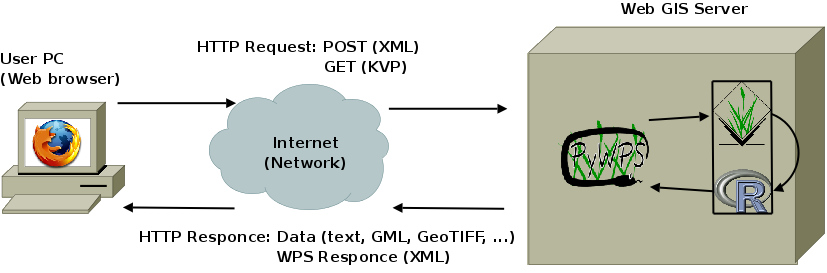
\includegraphics[width=1\textwidth]{pic/pywps-schema}
\caption{How does PyWPS work: GRASS GIS is in this case working tool}
\label{pic:pywps}
\end{center}
\end{figure}

%---------------------------------------------------------------------
\section{Quick install}
\begin{enumerate}
    \item Install PyWPS, see page~\pageref{install} for details
    \item NOTE: Rename original files (process examples, configuration files)
    with \texttt{.py-dist} suffix to \texttt{.py}, when you see them.
    \item Edit configuration files in \texttt{pywps/etc/} directory. See
    page~\pageref{configuration} for details.
    \item Create or edit \texttt{\_\_init\_\_.py} file in
    \texttt{pywps/processes} directory. Add available process names to
    \texttt{\_\_all\_\_} array.
    \item Add your processes to \texttt{pywps/processes} directory. See
    page~\pageref{processes} for details.
    \item Run PyWPS with \texttt{./wps.py} command, see
    page~\pageref{testing} for details.
\end{enumerate}

    
%---------------------------------------------------------------------
\section{Know issues}
Known bugs and limitations to \date
\begin{itemize}
\item Translations do not work for GetCapabilities. They only work for DescribeProcess request types.
\item If inputs are of type \texttt{LiteralValue} and it's type is
string, it could be security problem. Take care on your inputs and do
not use it directly in scripts to avoid your server to be hacked.
\end{itemize}

Please report all problems or unexpected handeling either via pywps mailing
list\footnote{\href{http://wald.intevation.org/mailman/listinfo/pywps-devel}{PyWPS
- development list}}
or using PyWPS
bugtracker\footnote{\href{http://wald.intevation.org/tracker/?atid=174&group\_id=22&func=browse}{PyWPS
Bug tracker}}.

%---------------------------------------------------------------------
\section{Installation}
\label{install}   
Required packages:
    
\begin{itemize}
    \item python 
    \item python-xml 
    \item python-htmltmpl 
\end{itemize}
    
Recommended packages:
    
\begin{itemize}
    \item Web Server (e.g. Apache) -- \url{http://httpd.apache.org} -  You
    will need an web server, to be able to execute processes from remote
    computers.

    \item GIS GRASS  -- \url{http://grass.itc.it} - Geographical Resources
    Analysis Support System (GRASS) is Open Source GIS, which provides more
    then 350 modules for raster and vector (2D, 3D) data analysis. PyWPS is
    written with native support for GRASS and it's functions.

    \item PROJ.4  -- \url{http://proj.maptools.org} - Cartographic
    Projections library used in various Open Source projects, such as
    GRASS, UMN MapServer, QGIS and others. It can be used e.g. for data
    transformation.

    \item GDAL/OGR  -- \url{http://gdal.org} - translator library for
    raster geospatial data formats, is used in various projects for
    importing, exporting and transformation between various raster and vector
    data formats.

    \item R  -- \url{http://www.r-project.org} - is a language and environment
    for statistical computing and graphics.

\end{itemize}
    
\subsection{Installation the quick 'n' dirty way}
For installing pywps to your server simply unzip the archive to the
directory, where cgi programs are allowed to run. You can also use current
repository version.

\begin{verbatim}
$ cd /usr/lib/cgi-bin/
$ tar xvzf /tmp/pywps-VERSION.tar.gz
$ pywps/wps.py
\end{verbatim}

\subsection{Installation the 'clean' way}
Unzip the package 
\begin{verbatim}
$ tar -xzf pywps-VERSION.tar.gz
\end{verbatim}
and run 
\begin{verbatim}
$ python setup.py install
\end{verbatim} 
adjust the configuration file 
\begin{verbatim}
$ vim /etc/pywps.cfg
\end{verbatim} 
permint write access to templates directory
\begin{verbatim}
# chmod -R 777 /usr/lib/python2.5/site-packages/pywps/Templates
\end{verbatim} 

Several binary packages for Linux distributios (\texttt{RPM,DEB}) are also avaliable on PyWPS
homepage\footnote{\pywpssite}.

%---------------------------------------------------------------------
\section{Configuration}
\label{configuration}
    
Before you start to tune your PyWPS installation, you should get your copy of
OpenGIS(R) Web Processing Service document (OGC  05-007r7) version
1.0.0\footnote{\url{http://www.opengeospatial.org/standards/wps}}.
    
\note{Note, that the configuration option are CASE SENSITIVE}
    
Pywps configuration takes place in \texttt{pywps.cfg} file located in
\texttt{/etc/pywps.cfg} or \texttt{pywps/etc/pywps.cfg}. 

Default configuration file is located in \texttt{pywps/default.cfg}, you
can always make a copy of this file and start the configuration from
scratch.
    
Several sections are in the file. 
\begin{itemize}
    \item Section \textbf{[wps]} contains general WPS settings, which are:
        \begin{itemize}
            \item encoding -- Language encoding (utf-8, iso-8859-2, windows-1250, \dots)
            \item title -- Server title 
            \item version -- WPS version (1.0.0)
            \item abstract -- Server anstract
            \item fees -- Possible fees
            \item constraints -- Possible constraints
            \item serveraddress -- WPS script address: \url{http://foo/bar/wps.py}
            \item keywords -- Comma-separated list of kyewords
            \item lang -- Default langue (eng)
        \end{itemize}
    \item Section \textbf{[provider]} contains informations about you
        \begin{itemize}
            \item providerName -- Name of your company
            \item individualName -- Your name
            \item positionName
            \item role 
            \item deliveryPoint -- Street
            \item city
            \item postalCode
            \item country
            \item electronicMailAddress -- foo@bar
            \item providerSite -- \url{http://foo.bar}
            \item phoneVoice
            \item phoneFacsimile
            \item administrativeArea
        \end{itemize}
    \item Section \textbf{[server]} contains server settings
        \begin{itemize}
            \item maxoperations -- Maximal number of parallel running
            processes. If set to 0, then there is no limit.
            \item maxinputparamlength -- Maximal length of string input
            parameter.
            \item maxfilesize -- Maximal input file size (raster or
            vector). The size can be determined as follows: 1GB, 5MB, 3kB,
            1000b.
            \item tempPath -- Direcotory for temporary files (mostly
            temporary GRASS locations).
            \item outputUrl -- Url where the outputs are stored.
            \item outputPath -- Path. where output files are stored.
            \item debug -- true/false
        \end{itemize}
    \item Section \textbf{[grass]} -- GRASS GIS settings
        \begin{itemize}
            \item path -- \$PATH variable, e.g. \texttt{/usr/lib/grass/bin}
            \item addonPath -- \$GRASS\_ADDONS variable
            \item version -- GRASS version
            \item gui -- Should be "text"
            \item gisbase -- Path to GRASS GIS\_BASE directory
            (\texttt{/usr/lib/grass})
            \item ldLibraryPath -- Path of GRASS Libs
            (\texttt{/usr/lib/grass/lib})
        \end{itemize}
\end{itemize}

File example follows:
\begin{verbatim}
[wps]
encoding=utf-8
title=PyWPS Server
version=1.0.0
abstract=See http://pywps.wald.intevation.org and http://www.opengeospatial.org/standards/wps
fees=None
constraints=none
serveraddress=http://localhost/cgi-bin/wps
keywords=GRASS,GIS,WPS
lang=eng

[provider]
providerName=Your Company Name
individualName=Your Name
positionName=Your Position
role=Your role
deliveryPoint=Street
city=City
postalCode=000 00
country=eu
electronicMailAddress=login@server.org
providerSite=http://foo.bar
phoneVoice=False
phoneFacsimile=False
administrativeArea=False

[server]
maxoperations=3
maxinputparamlength=1024
maxfilesize=3mb
tempPath=/tmp
outputUrl=http://localhost/wps/wpsoutputs
outputPath=/var/www/wps/wpsoutputs
debug=true

[grass]
path=/usr/lib/grass/bin/:/usr/lib/grass/scripts/
addonPath=
version=6.2.1
gui=text
gisbase=/usr/lib/grass/
ldLibraryPath=/usr/lib/grass/lib
\end{verbatim}
    
subsection{Testing after installation}
\label{testing}
For test, just run
\texttt{wps.py} in your command line:
    
\begin{verbatim}
$ ./wps.py "service=wps&request=getcapabilities"

INIT DONE
LOADING PRECOMPILED
TEMPLATE: UPTODATE
PRECOMPILED: UPTODATE
Content-type: text/xml

<?xml version="1.0" encoding="utf-8"?>
<wps:Capabilities service="WPS" version="1.0.0" xml:lang="eng,ger"
    xmlns:xlink="http://www.w3.org/1999/xlink"
    xmlns:wps="http://www.opengis.net/wps/1.0.0"
    xmlns:ows="http://www.opengis.net/ows/1.1"
    xmlns:xsi="http://www.w3.org/2001/XMLSchema-instance
    xsi:schemaLocation="http://www.opengis.net/wps/1.0.0
    http://schemas.opengis.net/wps/1.0.0/wpsGetCapabilities_response.xsd"
    updateSequence="1">
	<ows:ServiceIdentification>
		<ows:Title>PyWPS Development Server</ows:Title>
    ...
</wps:Capabilities>
\end{verbatim}

If you got something like this, (Capabilities response), everything looks
fine.
     
If you got some other message, like e.g.:
     
\begin{verbatim}
Traceback (most recent call last):
  File "/usr/bin/wps.py", line 221, in <module>
    wps = WPS()
  File "/usr/bin/wps.py", line 140, in __init__
    self.performRequest()
  File "/usr/bin/wps.py", line 188, in performRequest
    from pywps.WPS.GetCapabilities import GetCapabilities
  File "/usr/lib/python2.5/site-packages/pywps/WPS/GetCapabilities.py", line 26, in <module>
    from Response import Response
  File "/usr/lib/python2.5/site-packages/pywps/WPS/Response.py", line 28, in <module>
    from htmltmpl import TemplateManager, TemplateProcessor
ImportError: No module named htmltmpl
\end{verbatim}

     
Than something is wrong with your Python installation or with the program.
This message means, that the python-htmltmpl package is not installed in
your system.
     
%---------------------------------------------------------------------
\section{Write your own processes}
\label{processes}
    
All processes are stored in the \texttt{pywps/processes} directory. You can
create custom directory anywhere in your system and set
\texttt{\$PYTHON\_PROCESS} environment variabl (how to do this for the web
server, refer to your Server documentation). Following example will
describe buffering process.  Several example processes are distributed along with PyWPS source code.

Create file \texttt{exampleBufferProcess.py} in PYWPS\_PROCESSES directory.
    
Each process is stand-alone python script with one class \texttt{Process},
which has two methods: \texttt{\_\_init\_\_, execute}. It is possible also to add as 
many your functions/methods, as you wish.
    
\subsection{Process initialization and configuration}

\begin{verbatim}
  1 from pywps.Process.Process import WPSProcess                                
  2 class Process(WPSProcess):
  3     """Main process class"""
  4     def __init__(self):
  5         """Process initialization"""
  7         # init process
  8         WPSProcess.__init__(self,
  9             identifier = "exampleBufferProcess",
 10             title="Buffer",
 11             version = "0.2",
 12             storeSupported = "true",
 13             statusSupported = "true",
 14             abstract="Create a buffer around an input vector file",
 15             grassLocation = True)
\end{verbatim}

We defined new process called \texttt{exampleBufferProcess}. The process is allowed to
store it's output data on the server (\texttt{storeSupported}) and it is also possible to run it in
asynchronous mode (\texttt{statusSupported}). The process will run within
GRASS GIS environment (\texttt{grassLocation = True}).
     
\paragraph{Metadata defition} is stored in array \texttt{self.Metadata} in
\texttt{\_\_init\_\_} method. You can add new Medatada using
\texttt{self.AddMetadata()} method:
\begin{verbatim}
            self.AddMetadata(identifier="point",type="point",
                            textContent="Click in the map")
\end{verbatim}

\subsubsection{Data Inputs}

Three types of data inputs are defined:
\begin{itemize}
    \item Literal Input -- Basic literal input -- single number or text
    value
    \item ComplexValue Input  -- Mostly vector file embded in input XML
    request or reference (URL) to such file.
    \item BoundingBox Input -- Coordinates for lower-left and upper-right
    corner.
\end{itemize}


\paragraph{ComplexInput}
Complex input can be raster or vector file, to be processed. 

\begin{verbatim}
 18         self.dataIn = self.addComplexInput(identifier="data",
 19                              title = "Input data")
 20 
\end{verbatim}

\paragraph{LiteralInput}

With literal input, you can obtain any type of character string.

\begin{verbatim}
 21         self.widthIn = self.addLiteralInput(identifier = "width",
 22                              title = "Width")
 23 
\end{verbatim}

For further documentation, refere example processes distributed with the
source code as well as \texttt{pydoc~pywps/Wps/Process.py}. This help is
also available in
\texttt{process.html}\footnote{\href{http://wald.intevation.org/plugins/scmsvn/viewcvs.php/*checkout*/trunk/doc/process.html?rev=369&root=pywps}{Documentation
to Process.py module}} file distributed along with PyWPS
source code.

\subsubsection{Data Outputs}
Data outputs can be defined in similar way.
\begin{itemize}
    \item Literal Output
    \item ComplexValue Outout
    \item BoundingBox Output
\end{itemize}
    
\paragraph{ComplexValue Output}
The complex value can be raster or vector file (or any other binary or text
file).

\begin{verbatim}
24        self.bufferOut = self.addComplexOutput(identifier="buffer",
25                                title="Output buffer file")
26
\end{verbatim}

\paragraph{Literal Output}
If you want to output any text string.
\begin{verbatim}
27          self.textOut = self.addLiteralOutput(identifier="text",
28                               title="just some text")
29
\end{verbatim}

\subsection{Process Programming}
    
The process must be defined in the \texttt{execute(self)} method. 
Basicly, you want to get input values and set output values. For this
purpose, you can use \texttt{getValue(input\_identifier)} and
\texttt{setValue(output\_identifier,value)} methods of the input/output
objects (see lower).

If you need to execute some shell command, you should use
\texttt{self.cmd(command,["string for standard input"])} instead of e.g.
\texttt{os.system()} or \texttt{os.popen()} functions.

Calculation progress can be set using \texttt{self.status(string message,
number percent)} method.

Example follows:

\begin{verbatim}
33     def execute(self):
34         """Execute process.
35         
36         Each command will be executed and output values will be set
37         """
38 
39         # run some command from the command line
40         self.cmd("g.region -d")
41 
42         # set status value
43         self.status.set("Importing data",20)
44         self.cmd("v.in.ogr dsn=%s output=data" %\
45                 (self.getInputValue('data')))
46             
47         self.status.set("Buffering",50)
48         self.cmd("v.buffer input=data output=data_buff buffer=%s scale=1.0 tolerance=0.01" %\
49                 (self.getInputValue('width')))
50 
51         self.status.set("Exporting data",90)
52 
53         self.cmd("v.out.ogr type=area format=GML input=data_buff dsn=out.xml olayer=path.xml")
54         
55         self.bufferOut.setValue("out.xml")
56         self.textOut.setValue("ahoj, svete")
57         return
\end{verbatim}

\subsubsection{Error handling}
    
At the end of the \texttt{execute} function, \texttt{None} value should be returned. Any other 
value means, that the calculation will be stopped and error report will be
returned back to the client, example:

\begin{verbatim}
        def execute(self):
            ...
            return "Ups, something failed!"
\end{verbatim}
    

\subsection{Using GRASS GIS}

Configuration is done using standard pywps configuration file (see
page\pageref{configuration}).


If you want to use GRASS GIS commands in your process, and there is no
GRASS Location to be used, you have to set \texttt{grassLocation=True} in
process definition:

\begin{verbatim}
         WPSProcess.__init__(self,
             identifier = "exampleBufferProcess",
             ....
             grassLocation = True)
\end{verbatim}

In this case, temporary GRASS Location will be created and after the
process is done, it will be deleted again. By default, no GRASS Location is
created.

You can also work in existing GRASS Location, then just set the location
path:
\begin{verbatim}
         WPSProcess.__init__(self,
             identifier = "exampleBufferProcess",
             ....
             grassLocation = "/home/grass/grassdata/spearfish60")
\end{verbatim}

%---------------------------------------------------------------------
\section{Testing your new process}

To test your PyWPS installation, you run it either as Webserver
cgi-application or in the command line directly. It is always good to start
with the command line test, so do not have to check \texttt{error.log} of
the web server.

\begin{itemize}
    \item GetCapabilities request (webserver)
\begin{verbatim}
./wps.py "service=wps&request=getcapabilities"

wget -nv -q -O - "http://localhost/cgi-bin/wps.py?\
    service=Wps&request=getcapabilities"
\end{verbatim}
        
    \item DescribeProcess request:
\begin{verbatim}
./wps.py "version=1.0.0&service=Wps&request=DescribeProcess&\
    Identifier=bufferExampleProcess"

wget -nv -q -O - "http://localhost/cgi-bin/wps.py?\
    version=0.4.0&service=Wps&request=DescribeProcess&\
    Identifier=exampleBufferProcess"
\end{verbatim}
        
    \item Execute request:
            For data inputs encoding, using HTTP Get method, see
            \pywpsDocCurrent, page 38 ,,Execute HTTP GET request KVP
            encoding``
\begin{verbatim}
./wps.py "version=1.0.0&service=Wps&\
    request=Execute&Identifier=exampleBufferProcess&\
    datainputs=data=http://foo/bar/roads.gml;width=0.5"
\end{verbatim}
        
\end{itemize}


Some examples of XML request econding are available in doc/examples
directory.

Before testing WPS via HTTP POST, you have to set \texttt{REQUEST\_METHOD}
environment variable, then you can redirect input XML into \texttt{wps.py}
script via standard input:

\begin{verbatim}
$ export REQUEST_METHOD=POST
$ cat doc/wps_execute_request-responsedocument.xml|./wps.py
\end{verbatim}

\end{document}
